% ==================================================================
%  徐森林、金亚东、薛春华《数学分析》（第三册）
%  S13.2  极限函数与和函数的重要性质
%  源：原书印刷页 101-128（PDF 物理页 107-134）
%  底本：PaddleOCR-VL-1.6，见 chapters/_ch13_13_2_raw.md
%  约定：全西文标点；行间公式用一对方括号；多行公式用 align/aligned；
%        跨册引用一律 \extref；数学模式内的中文必须包 \text{}
%  插图：图 13.2.1-13.2.7 原生 TikZ 绘制（禁用位图）
%  带撇编号：定理 13.2.1'-13.2.5'、推论 13.2.1'-13.2.4'
%           均用 *p 环境 + \setcounter 手工拨号（见 _make_ch13_2b.py）
%  已订正的 OCR 错误与原书照录清单见 tools/_make_ch13_2a.py 头部说明
% ==================================================================
\section{极限函数与和函数的重要性质}\label{sec:13.2}

回顾 13.1 节中提出的 3 个问题, 我们将看到, 只要加上一致收敛的条件, 所提问题的答案都是肯定的.

\begin{theorem}\label{thm:13.2.1}
设 $\{f_{n}(x)\}$ 在 $I\subset\mathbb{R}$ 上为连续函数列, 且 $\{f_{n}(x)\}$ 在 $I$ 上一致收敛于函数 $f(x)$, 则 $f(x)$ 在 $I$ 上为连续函数.
\end{theorem}

\begin{proof}
$\forall x_{0}\in I$, 由于 $\{f_{n}(x)\}$ 在 $I$ 上一致收敛于 $f(x)$, 故 $\forall\varepsilon>0$, $\exists N\in\mathbb{N}$, 使得
\[
  |f_{N}(x)-f(x)|<\frac{\varepsilon}{3},\quad\forall x\in I.
\]
因为 $f_{N}(x)$ 为 $I$ 上的连续函数, 所以它在 $x_{0}$ 处连续, 故 $\exists\delta>0$, 当 $x\in I$ 且 $|x-x_{0}|<\delta$ 时, 有
\[
  |f_{N}(x)-f_{N}(x_{0})|<\frac{\varepsilon}{3}.
\]
于是, 当 $x\in I$ 且 $|x-x_{0}|<\delta$, 有
\[
  \begin{aligned}
    |f(x)-f(x_{0})|&\leqslant|f(x)-f_{N}(x)|+|f_{N}(x)-f_{N}(x_{0})|+|f_{N}(x_{0})-f(x_{0})|\\
    &<\frac{\varepsilon}{3}+\frac{\varepsilon}{3}+\frac{\varepsilon}{3}=\varepsilon.
  \end{aligned}
\]
这就证明了 $f(x)$ 在 $x_{0}$ 处连续. 由于 $x_{0}$ 是 $I$ 的任意点, 所以 $f(x)$ 在 $I$ 上连续.
\end{proof}

\begin{corollary}\label{cor:13.2.1}
设 $\{f_{n}(x)\}$ 在 $I\subset\mathbb{R}$ 上为连续函数列, 且 $\{f_{n}(x)\}$ 在 $I$ 上收敛于函数 $f(x)$, 如果 $f(x)$ 在 $I$ 上不为连续函数, 则 $\{f_{n}(x)\}$ 在 $I$ 上不一致收敛.
\end{corollary}

\begin{proof}
(反证) 假设 $\{f_{n}(x)\}$ 在 $I$ 上一致收敛, 根据定理~\ref{thm:13.2.1} 知, $f(x)$ 为 $I$ 上的连续函数, 这与题设 $f(x)$ 在 $I$ 上不为连续函数相矛盾.
\end{proof}

推论~\ref{cor:13.2.1} 是证明函数列 $\{f_{n}(x)\}$ 在 $I$ 上不一致收敛的最简单且应首选的方法. 例如: $f_{n}(x)=x^{n}$, $x\in(0,1]$ 都连续, 但
\[
  f(x)=\lim_{n\to+\infty}f_{n}(x)=\begin{cases}
    0, & x\in(0,1),\\
    1, & x=1
\end{cases}
\]
不连续, 根据推论~\ref{cor:13.2.1} 知, $\{f_{n}(x)\}$ 在 $I=(0,1]$ 上不一致收敛.

但是, 如果 $f(x)$ 在 $I$ 上连续, 推论~\ref{cor:13.2.1} 就无能为力了.

更一般地, 有下面的结论.

\begin{theorem}\label{thm:13.2.2}
设 $I\subset\mathbb{R}$, $\{f_{n}(x)\}$ 在 $I$ 上一致收敛, $x_{0}\in I'\setminus I$, $\lim\limits_{x\to x_{0}}f_{n}(x)=c_{n}$, $\forall n\in\mathbb{N}$. 则 $\{c_{n}\}$ 收敛于 $c\in\mathbb{R}$, 且
\[
  \lim_{x\to x_{0}}f(x)=\lim_{n\to+\infty}\lim_{x\to x_{0}}f_{n}(x)=\lim_{n\to+\infty}c_{n}=c.
\]
\end{theorem}

\begin{proof}
因为 $\{f_{n}(x)\}$ 在 $I$ 上一致收敛, 所以 $\forall\varepsilon>0$, $\exists N=N(\varepsilon)\in\mathbb{N}$, 当 $m,n>N$, 有
\[
  |f_{n}(x)-f_{m}(x)|<\frac{\varepsilon}{2},
\]
令 $x\to x_{0}$ 得到
\[
  |c_{n}-c_{m}|=\lim_{x\to x_{0}}|f_{n}(x)-f_{m}(x)|\leqslant\frac{\varepsilon}{2}<\varepsilon.
\]
这就表明 $\{c_{n}\}$ 为 Cauchy 数列. 它收敛于 $c$, 即 $\lim\limits_{n\to+\infty}c_{n}=c\in\mathbb{R}$.

进一步, $\forall\varepsilon>0$, 因为 $\lim\limits_{n\to+\infty}c_{n}=c$, 所以 $\exists N_{1}\in\mathbb{N}$, 当 $n>N_{1}$ 时, $|c_{n}-c|<\frac{\varepsilon}{3}$. 另一方面, 由 $\{f_{n}(x)\}$ 在 $I$ 上一致收敛, 故 $\exists N_{2}\in\mathbb{N}$, 使得当 $n>N_{2}$ 时, 有
\[
  |f_{n}(x)-f(x)|<\frac{\varepsilon}{3},\quad\forall x\in I.
\]
于是, 令 $N=\max\{N_{1},N_{2}\}+1$, 因 $\lim\limits_{x\to x_{0}}f_{N}(x)=c_{N}$, 故 $\exists\delta>0$, 当 $0<|x-x_{0}|<\delta$, $x\in I$, 有 $|f_{N}(x)-c_{N}|<\frac{\varepsilon}{3}$, 且
\[
  \begin{aligned}
    |f(x)-c|&\leqslant|f(x)-f_{N}(x)|+|f_{N}(x)-c_{N}|+|c_{N}-c|\\
    &<\frac{\varepsilon}{3}+\frac{\varepsilon}{3}+\frac{\varepsilon}{3}=\varepsilon.
  \end{aligned}
\]
这就证明了 $\lim\limits_{x\to x_{0}}f(x)=c$.
\end{proof}

用反证法及定理~\ref{thm:13.2.2} 立即有下面的推论.

\begin{corollary}\label{cor:13.2.2}
设 $I\subset\mathbb{R}$, $x_{0}\in I'\setminus I$, 如果
\[
  \lim_{x\to x_{0}}\lim_{n\to+\infty}f_{n}(x)\neq\lim_{n\to+\infty}\lim_{x\to x_{0}}f_{n}(x)
\]
则 $\{f_{n}(x)\}$ 在 $I$ 上不一致收敛.
\end{corollary}

\begin{remark}\label{rem:13.2.1}
定理~\ref{thm:13.2.2} 中 ``$x_{0}$'' 改为 ``$x_{0}^{+}$ 或 $x_{0}^{-}$ 或 $+\infty$ 或 $-\infty$ 或 $\infty$'' 结论仍成立.
\end{remark}

\begin{example}\label{ex:13.2.1}
证明: 函数列
\[
  f_{n}(x)=\begin{cases}
    1-nx, & 0\leqslant x\leqslant\frac{1}{n},\\
    0, & \frac{1}{n}<x\leqslant1
\end{cases}
\]
在 $[0,1]$ 上不一致收敛 (\cref{fig:13.2.1}).
\end{example}

\begin{proof}
证法 1 显然
\[
  f(x)=\begin{cases}
    1, & x=0,\\
    0, & 0<x\leqslant1.
\end{cases}
\]
\[
  \begin{aligned}
    \lim_{x\to0^{+}}f(x)&=\lim_{x\to0^{+}}\lim_{n\to+\infty}f_{n}(x)=0\neq1=\lim_{n\to+\infty}1\\
    &=\lim_{n\to+\infty}\lim_{x\to0^{+}}(1-nx)=\lim_{n\to+\infty}\lim_{x\to0^{+}}f_{n}(x)=\lim_{n\to+\infty}f_{n}(0)=f(0).
  \end{aligned}
\]
根据定理~\ref{thm:13.2.2} 或推论~\ref{cor:13.2.1} 知, $\{f_{n}(x)\}$ 在 $[0,1]$ 上不一致收敛.

证法 2 (反证) 假设 $\{f_{n}(x)\}$ 在 $[0,1]$ 上一致收敛于 $f(x)$, 则对 $\varepsilon=\frac{1}{2}$, $\exists N\in\mathbb{N}$, 当 $n>N$ 时, 有
\[
  |f_{n}(x)-f(x)|<\varepsilon=\frac{1}{2},\quad\forall x\in[0,1].
\]
显然
\[
  \frac{1}{2}=\left|\left(1-n\cdot\frac{1}{2n}\right)-0\right|<\varepsilon=\frac{1}{2},
\]
矛盾.
\end{proof}

\begin{figure}[htbp]
  \centering
  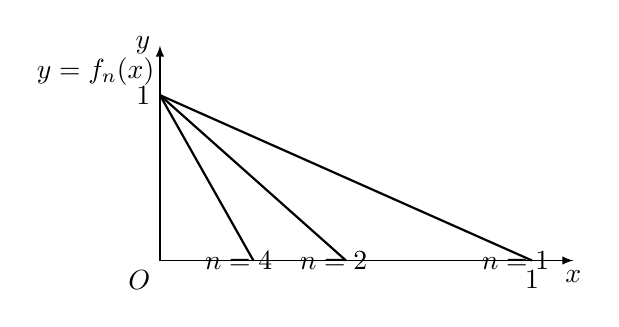
\begin{tikzpicture}[>=latex, scale=1.05]
    \draw[->] (0,0) -- (5.00,0) node[below] {$x$};
    \draw[->] (0,0) -- (0,2.60) node[left] {$y$};
    \node[below left] at (0,0) {$O$};
    \node[below] at (4.50,0) {$1$};
    \node[left] at (0,2.00) {$1$};
    % f_1: 1-x  (零点 x=1)
    \draw[thick] (0,2.00) -- (4.50,0);
    % f_2: 1-2x (零点 x=1/2)
    \draw[thick] (0,2.00) -- (2.25,0);
    % f_4: 1-4x (零点 x=1/4)
    \draw[thick] (0,2.00) -- (1.13,0);
    \node[above left] at (0.05,2.00) {$y=f_{n}(x)$};
    \node[below] at (4.30,0.22) {$n=1$};
    \node[below] at (2.10,0.22) {$n=2$};
    \node[below] at (0.95,0.22) {$n=4$};
  \end{tikzpicture}
  \caption{$f_{n}(x)=1-nx$ ($0\leqslant x\leqslant1/n$)}\label{fig:13.2.1}
\end{figure}

\begin{theorem}\label{thm:13.2.3}
如果 $[a,b]$ 上的 Riemann 可积函数列 (特别是连续函数列) $\{f_{n}(x)\}$ 在 $[a,b]$ 上一致收敛于 $f(x)$, 则 $f(x)$ 在 $[a,b]$ 上也 Riemann 可积 (连续), 且
\[
  \lim_{n\to+\infty}\int_{a}^{b}f_{n}(x)\mathrm{d}x=\int_{a}^{b}f(x)\mathrm{d}x.
\]
\end{theorem}

\begin{proof}
(参阅\extref{定理 6.3.6}) 先证 $f(x)$ 在 $[a,b]$ 上 Riemann 可积. 由于 $f_{n}(x)$ 在 $[a,b]$ 上 Riemann 可积, 根据 Lebesgue 定理 6.1.4(8), $D_{\text{不}}(f_{n})$ 为零测度集. 从定理~\ref{thm:13.2.1} 的证明或定理~\ref{thm:13.2.2}, 有
\[
  D_{\text{不}}(f(x))\subset\bigcup_{n=1}^{\infty}D_{\text{不}}(f_{n}(x)).
\]
再由\extref{引理 6.1.6}(4) 及 (2) 立即推得 $D_{\text{不}}(f(x))$ 为零测度集. 因为 $\{f_{n}(x)\}$ 在 $[a,b]$ 上一致收敛于 $f(x)$, 故 $\exists N_{0}\in\mathbb{N}$, 使得
\[
  |f(x)-f_{N_{0}}(x)|<1,\quad\forall x\in[a,b].
\]
又因 $f_{N_{0}}(x)$ 为有界函数, 不妨设 $|f_{N_{0}}(x)|\leqslant M$, $\forall x\in[a,b]$. 于是
\[
  |f(x)|\leqslant|f_{N_{0}}(x)|+1\leqslant M+1,\quad\forall x\in[a,b],
\]
即 $f(x)$ 在 $[a,b]$ 上为有界函数.

综合上述及由 Lebesgue 定理 6.1.4(8) 知 $f(x)$ 在 $[a,b]$ 上也 Riemann 可积.

另一方面, 由于 $\{f_{n}(x)\}$ 在 $[a,b]$ 上一致收敛于 $f(x)$, 故 $\forall\varepsilon>0$, $\exists N=N(\varepsilon)\in\mathbb{N}$, 当 $n>N$ 时, 有
\[
  |f_{n}(x)-f(x)|<\varepsilon,\quad\forall x\in[a,b].
\]
\[
  \begin{aligned}
    \left|\int_{a}^{b}f_{n}(x)\mathrm{d}x-\int_{a}^{b}f(x)\mathrm{d}x\right|&=\left|\int_{a}^{b}[f_{n}(x)-f(x)]\mathrm{d}x\right|\\
    &\leqslant\int_{a}^{b}|f_{n}(x)-f(x)|\mathrm{d}x<\varepsilon(b-a),
  \end{aligned}
\]
\[
  \lim_{n\to+\infty}\int_{a}^{b}f_{n}(x)\mathrm{d}x=\int_{a}^{b}f(x)\mathrm{d}x=\int_{a}^{b}\lim_{n\to+\infty}f_{n}(x)\mathrm{d}x.
\]
\end{proof}

用反证法及定理~\ref{thm:13.2.3} 立即有下面的推论.

\begin{corollary}\label{cor:13.2.3}
设 $\{f_{n}(x)\}$ 为 $[a,b]$ 上的 Riemann 可积函数, 如果
\[
  \lim_{n\to+\infty}\int_{a}^{b}f_{n}(x)\mathrm{d}x\neq\int_{a}^{b}f(x)\mathrm{d}x,
\]
则 $\{f_{n}(x)\}$ 在 $[a,b]$ 上不一致收敛.
\end{corollary}

\begin{example}[参阅例~\ref{ex:13.1.7}]\label{ex:13.2.2}
设 $\mathbb{Q}\cap[0,1]=\{r_{1},r_{2},\cdots,r_{n},\cdots\}$ 是 $[0,1]$ 上的全体有理数, 而
\[
  S_{n}(x)=\begin{cases}1, & x=r_{1},\cdots,r_{n},\\ 0, & x\text{ 为其他值},\end{cases}\qquad
  S(x)=\begin{cases}1, & x\text{ 为有理数},\\ 0, & x\text{ 为无理数}.\end{cases}
\]
显然, $\lim\limits_{n\to+\infty}S_{n}(x)=S(x)$, 且每个 $S_{n}(x)$ 在 $[0,1]$ 上是只有有限个不连续点的有界函数, 它是 Riemann 可积的. 因为 $S(x)$ 在 $[0,1]$ 上处处不连续, 所以它在 $[0,1]$ 上非 Riemann 可积.
\end{example}

现证 $\{S_{n}(x)\}$ 在 $[0,1]$ 上不一致收敛于 $S(x)$. (反证) 假设 $\{S_{n}(x)\}$ 在 $[0,1]$ 上一致收敛于 $S(x)$. 根据定理~\ref{thm:13.2.3}, $S(x)$ 在 $[0,1]$ 上必 Riemann 可积, 这与上述非 Riemann 可积相矛盾.

\begin{example}[参阅\extref{例 6.3.12}]\label{ex:13.2.3}
设 (\cref{fig:13.2.2})
\[
  f_{n}(x)=\begin{cases}
    4n^{2}x, & 0\leqslant x\leqslant\frac{1}{2n},\\
    -4n^{2}x+4n, & \frac{1}{2n}<x\leqslant\frac{1}{n},\\
    0, & \frac{1}{n}<x\leqslant1,
\end{cases}
\]
则 $f(x)=\lim\limits_{n\to+\infty}f_{n}(x)=0$. 下面证明 $\{f_{n}(x)\}$ 在 $[0,1]$ 上不一致收敛于 $f(x)=0$.
\end{example}

因为 $f(x)=0$ 连续、Riemann 可积, 故不能应用定理~\ref{thm:13.2.1} 或定理~\ref{thm:13.2.2} 或定理~\ref{thm:13.2.3} 及反证法证明 $\{f_{n}(x)\}$ 在 $[0,1]$ 上不一致收敛. 也就是不能对 $\{f_{n}(x)\}$ 在 $[0,1]$ 上是否一致收敛于 $f(x)=0$ 给出任何信息.

\begin{proof}
证法 1 (反证) 假设 $\{f_{n}(x)\}$ 在 $[0,1]$ 上一致收敛于 $f(x)=0$, 则由定理~\ref{thm:13.2.3}, 有
\[
  \begin{aligned}
    1&=\lim_{n\to+\infty}\frac{1}{2}\cdot2n\cdot\frac{1}{n}=\lim_{n\to+\infty}\int_{0}^{1}f_{n}(x)\mathrm{d}x\\
    &=\int_{0}^{1}\lim_{n\to+\infty}f_{n}(x)\mathrm{d}x=\int_{0}^{1}f(x)\mathrm{d}x=\int_{0}^{1}0\mathrm{d}x=0,
  \end{aligned}
\]
矛盾.

证法 2 (反证) 假设 $\{f_{n}(x)\}$ 在 $[0,1]$ 上一致收敛于 $f(x)=0$, 则对 $\varepsilon=\frac{1}{2}$, $\exists N\in\mathbb{N}$, 当 $n>N$ 时, 有
\[
  |f_{n}(x)-f(x)|<\varepsilon=\frac{1}{2},\quad\forall x\in[0,1].
\]
显然
\[
  2\leqslant2n=\left|4n^{2}\cdot\frac{1}{2n}-0\right|<\varepsilon=\frac{1}{2},
\]
矛盾.
\end{proof}

\begin{figure}[htbp]
  \centering
  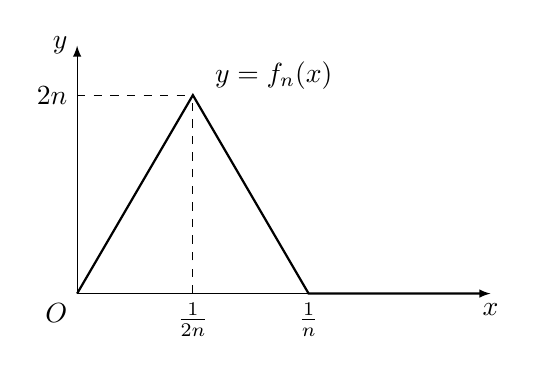
\begin{tikzpicture}[>=latex, scale=1.05]
    \draw[->] (0,0) -- (5.00,0) node[below] {$x$};
    \draw[->] (0,0) -- (0,3.00) node[left] {$y$};
    \node[below left] at (0,0) {$O$};
    \draw[thick] (0,0) -- (1.40,2.40) -- (2.80,0) -- (4.90,0);
    \draw[dashed] (1.40,0) -- (1.40,2.40);
    \draw[dashed] (0,2.40) -- (1.40,2.40);
    \node[below] at (1.40,0) {$\frac{1}{2n}$};
    \node[below] at (2.80,0) {$\frac{1}{n}$};
    \node[left] at (0,2.40) {$2n$};
    \node[above right] at (1.55,2.35) {$y=f_{n}(x)$};
  \end{tikzpicture}
  \caption{尖峰高 $2n$、底宽 $\frac{1}{n}$}\label{fig:13.2.2}
\end{figure}

\begin{example}\label{ex:13.2.4}
设 (\cref{fig:13.2.3})
\[
  f_{n}(x)=\begin{cases}
    2nx, & 0\leqslant x\leqslant\frac{1}{2n},\\
    2(1-nx), & \frac{1}{2n}<x\leqslant\frac{1}{n},\\
    0, & \frac{1}{n}<x\leqslant1,
\end{cases}
\]
则 $f(x)=\lim\limits_{n\to+\infty}f_{n}(x)=0$. 显然 $\{f_{n}(x)\}$ 在 $[0,1]$ 上一致有界 (以 $1$ 为界), 且
\[
  \begin{aligned}
    \lim_{n\to+\infty}\int_{0}^{1}f_{n}(x)\mathrm{d}x&=\lim_{n\to+\infty}\frac{1}{2}\cdot1\cdot\frac{1}{n}=0\\
    &=\int_{0}^{1}0\mathrm{d}x=\int_{0}^{1}f(x)\mathrm{d}x\\
    &=\int_{0}^{1}\lim_{n\to+\infty}f_{n}(x)\mathrm{d}x.
  \end{aligned}
\]
\end{example}

类似例~\ref{ex:13.2.3} 的理由, 因为 $f(x)=0$ 连续、Riemann 可积及
\[
  \lim_{n\to+\infty}\int_{0}^{1}f_{n}(x)\mathrm{d}x=\int_{0}^{1}\lim_{n\to+\infty}f_{n}(x)\mathrm{d}x
\]
都说明不能应用定理~\ref{thm:13.2.1} 或定理~\ref{thm:13.2.2} 或定理~\ref{thm:13.2.3} 及反证法证明 $\{f_{n}(x)\}$ 在 $[0,1]$ 上不一致收敛. 也就是不能对 $\{f_{n}(x)\}$ 在 $[0,1]$ 上是否一致收敛于 $f(x)=0$ 给出任何信息.

\begin{proof}
(反证) 假设 $\{f_{n}(x)\}$ 在 $[0,1]$ 上一致收敛于 $f(x)=0$, 则 $\varepsilon=\frac{1}{2}$, $\exists N\in\mathbb{N}$, 当 $n>N$ 时, 有
\[
  |f_{n}(x)-f(x)|<\varepsilon=\frac{1}{2},\quad\forall x\in[0,1].
\]
显然
\[
  1=|1-0|=\left|f_{n}\left(\frac{1}{2n}\right)-f\left(\frac{1}{2n}\right)\right|<\varepsilon=\frac{1}{2},
\]
矛盾.
\end{proof}

\begin{figure}[htbp]
  \centering
  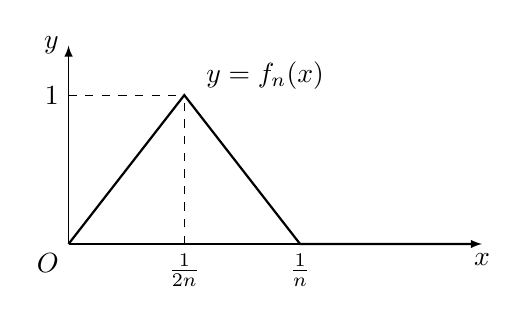
\begin{tikzpicture}[>=latex, scale=1.05]
    \draw[->] (0,0) -- (5.00,0) node[below] {$x$};
    \draw[->] (0,0) -- (0,2.40) node[left] {$y$};
    \node[below left] at (0,0) {$O$};
    \draw[thick] (0,0) -- (1.40,1.80) -- (2.80,0) -- (4.90,0);
    \draw[dashed] (1.40,0) -- (1.40,1.80);
    \draw[dashed] (0,1.80) -- (1.40,1.80);
    \node[below] at (1.40,0) {$\frac{1}{2n}$};
    \node[below] at (2.80,0) {$\frac{1}{n}$};
    \node[left] at (0,1.80) {$1$};
    \node[above right] at (1.55,1.75) {$y=f_{n}(x)$};
  \end{tikzpicture}
  \caption{尖峰高 $1$、底宽 $\frac{1}{n}$}\label{fig:13.2.3}
\end{figure}

\begin{theorem}\label{thm:13.2.4}
如果函数列 $\{f_{n}(x)\}$ 满足:

(1) 每一个 $f_{n}(x)$ 在 $[a,b]$ 上有连续的导函数;

(2) 由导函数构成的函数列 $\{f_{n}'(x)\}$ 在 $[a,b]$ 上一致收敛于函数 $g(x)$;

(3) 至少在某一点 $x_{0}\in[a,b]$ 收敛, 即 $\{f_{n}(x_{0})\}$ 收敛.

则函数列 $\{f_{n}(x)\}$ 在闭区间 $[a,b]$ 上一致收敛于某个连续可导的函数 $f(x)$, 且有
\[
  f'(x)=g(x),\quad\forall x\in[a,b],
\]
即
\[
  \lim_{n\to+\infty}f_{n}(x))'=\lim_{n\to+\infty}f_{n}'(x).
\]
\end{theorem}

\begin{proof}
因为 $\{f_{n}(x)\}$ 在 $x_{0}\in[a,b]$ 处收敛, 根据数列的 Cauchy 收敛准则, $\forall\varepsilon>0$, $\exists N_{1}\in\mathbb{N}$, 当 $n,m>N_{1}$ 时, 有
\[
  |f_{n}(x_{0})-f_{m}(x_{0})|<\frac{\varepsilon}{2}. \tag*{(1)}
\]
又因为 $\{f_{n}'(x)\}$ 在 $[a,b]$ 上一致收敛, 根据函数一致收敛的 Cauchy 收敛准则, $\exists N_{2}\in\mathbb{N}$, 当 $n,m>N_{2}$ 时, 有
\[
  |f_{n}'(x)-f_{m}'(x)|<\frac{\varepsilon}{2(b-a)},\quad\forall x\in[a,b]. \tag*{(2)}
\]
今 $N=\max\{N_{1},N_{2}\}$, 则当 $n,m>N$ 时, 不等式 (1) 与 (2) 成立.

由 Newton-Leibniz 公式, 有
\[
  f_{n}(x)=f_{n}(x_{0})+\int_{x_{0}}^{x}f_{n}'(t)\mathrm{d}t, \tag*{(3)}
\]
\[
  f_{m}(x)=f_{m}(x_{0})+\int_{x_{0}}^{x}f_{m}'(t)\mathrm{d}t,\quad\forall x\in[a,b]. \tag*{(4)}
\]
于是, 当 $n,m>N$ 时, 有
\[
  \begin{aligned}
    |f_{n}(x)-f_{m}(x)|&=\left|\left(f_{n}(x_{0})+\int_{x_{0}}^{x}f_{n}'(t)\mathrm{d}t\right)-\left(f_{m}(x_{0})+\int_{x_{0}}^{x}f_{m}'(t)\mathrm{d}t\right)\right|\\
    &=\left|f_{n}(x_{0})-f_{m}(x_{0})+\int_{x_{0}}^{x}[f_{n}'(t)-f_{m}'(t)]\mathrm{d}t\right|\\
    &\leqslant|f_{n}(x_{0})-f_{m}(x_{0})|+\left|\int_{x_{0}}^{x}|f_{n}'(t)-f_{m}'(t)|\mathrm{d}t\right|\\
    &<\frac{\varepsilon}{2}+\frac{\varepsilon}{2(b-a)}|x-x_{0}|\leqslant\varepsilon,\quad\forall x\in[a,b].
  \end{aligned}
\]
根据函数列一致收敛的 Cauchy 收敛准则, $\{f_{n}(x)\}$ 在 $[a,b]$ 上一致收敛. 设其极限函数为 $f(x)$.

由于 $\{f_{n}'(x)\}$ 在 $[a,b]$ 上一致收敛于 $g(x)$, $f_{n}'(x)$ 连续 ($\forall n\in\mathbb{N}$), 从定理~\ref{thm:13.2.1} 推得 $g(x)$ 在 $[a,b]$ 连续.

\[
  \lim_{n\to+\infty}\int_{x_{0}}^{x}f_{n}'(t)\mathrm{d}t\xlongequal{\text{定理~\ref{thm:13.2.3}}}\int_{x_{0}}^{x}\lim_{n\to+\infty}f_{n}'(t)\mathrm{d}t=\int_{x_{0}}^{x}g(t)\mathrm{d}t.
\]
在 (3) 式两边取 $n\to+\infty$ 得到
\[
  \lim_{n\to+\infty}f_{n}(x)=\lim_{n\to+\infty}\left[f_{n}(x_{0})+\int_{x_{0}}^{x}f_{n}'(t)\mathrm{d}t\right],
\]
即
\[
  f(x)=f(x_{0})+\int_{x_{0}}^{x}g(t)\mathrm{d}t.
\]
应用微积分的基本定理 6.3.2 即得
\[
  \lim_{n\to+\infty}f_{n}(x))'=f'(x)=g(x)=\lim_{n\to+\infty}f_{n}'(x).
\]
\end{proof}

用反证法及定理~\ref{thm:13.2.4} 立即有下面的推论.

\begin{corollary}\label{cor:13.2.4}
如果函数列 $\{f_{n}(x)\}$ 满足定理~\ref{thm:13.2.4} 中的 (1) 与 (3), 且
\[
  \lim_{n\to+\infty}f_{n}(x))'\neq\lim_{n\to+\infty}f_{n}'(x),
\]
则 $\{f_{n}'(x)\}$ 在 $[a,b]$ 上不一致收敛.
\end{corollary}

现在我们来考察定理~\ref{thm:13.2.1} 的逆定理是否成立, 即如果连续函数列 $\{f_{n}(x)\}$ 在 $[a,b]$ 上收敛于连续函数 $f(x)$, 问: $\{f_{n}(x)\}$ 在 $[a,b]$ 上是否一致收敛于 $f(x)$? 一般说来, 答案是否定的. 例~\ref{ex:13.2.3} 与例~\ref{ex:13.2.4} 都是反例. 如果附加条件: $\forall x\in[a,b]$, 数列 $\{f_{n}(x)\}$ 单调减收敛于 $0$, 则 $\{f_{n}(x)\}$ 在 $[a,b]$ 上一致收敛于 $f(x)$.

\begin{theorem}[Dini]\label{thm:13.2.5}
设函数列 $\{f_{n}(x)\}$ 在有界闭区间 $[a,b]$ 上连续, 如果 $\forall x\in[a,b]$, 数列 $\{f_{n}(x)\}$ 单调减收敛于 $0$, 则 $\{f_{n}(x)\}$ 在 $[a,b]$ 上一致收敛于 $f(x)=0$.
\end{theorem}

\begin{proof}
证法 1 $\forall\varepsilon>0$, $\exists N_{x}=N(x,\varepsilon)\in\mathbb{N}$, 使得
\[
  0\leqslant f_{N_{x}}(x)<\varepsilon.
\]
由于 $f_{N_{x}}(x)$ 在点 $x$ 连续, 必 $\exists\delta_{x}>0$, 使得当 $t\in[a,b]$ 且 $t\in(x-\delta_{x},x+\delta_{x})$ 时仍有
\[
  0\leqslant f_{N_{x}}(t)<\varepsilon.
\]
于是, 这些开区间 $\{(x-\delta_{x},x+\delta_{x})\mid x\in[a,b]\}$ 构成了 $[a,b]$ 的一个开覆盖. 根据 Heine-Borel 有限覆盖定理, 存在有限子覆盖 $\{(x_{i}-\delta_{x_{i}},x_{i}+\delta_{x_{i}})\mid i=1,2,\cdots,m\}$. 令 $N=\max\{N_{x_{1}},N_{x_{2}},\cdots,N_{x_{m}}\}$, 则当 $n>N$ 时, $\forall x\in[a,b]$, 必有 $x\in(x_{i}-\delta_{x_{i}},x_{i}+\delta_{x_{i}})$, 从而
\[
  0\leqslant f_{n}(x)\leqslant f_{N}(x)\leqslant f_{N_{x}}(x)<\varepsilon.
\]
这就证明了 $f_{n}(x)\rightrightarrows0=f(x)$, $x\in[a,b]$, $n\to+\infty$.

证法 2 (反证) 假设 $\{f_{n}(x)\}$ 在 $[a,b]$ 上不一致收敛于 $0$, 则 $\exists\varepsilon_{0}>0$, 使得 $\forall n\in\mathbb{N}$, 必有 $k_{n}>n$ 及 $x_{n}$ 满足 $f_{k_{n}}(x_{n})\geqslant\varepsilon_{0}$. 因为 $x_{n}\in[a,b]$, 根据 Bolzano-Weierstrass 的序列紧性定理, $\{x_{n}\}$ 有子列收敛于 $x_{0}\in[a,b]$, 这个子列仍记为 $\{x_{n}\}$. 此外, 可选 $k_{1}<k_{2}<\cdots<k_{n}<k_{n+1}<\cdots$. 由于 $\forall x\in[a,b]$, $\{f_{n}(x)\}$ 单调减少, 故当 $m>n$ 时, 有
\[
  f_{k_{n}}(x_{m})\geqslant f_{k_{m}}(x_{m})\geqslant\varepsilon_{0}.
\]
再从 $f_{n}(x)$ 连续推得
\[
  f_{k_{n}}(x_{0})=\lim_{n\to+\infty}f_{k_{n}}(x_{m})\geqslant\varepsilon_{0},
\]
\[
  0=\lim_{n\to+\infty}f_{k_{n}}(x_{0})\geqslant\varepsilon_{0}>0,
\]
矛盾.
\end{proof}

%  第二部分：定理 13.2.1' 起（生成脚本 tools/_make_ch13_2b.py）
% ==================================================================

%  第二部分：定理 13.2.1' 起（生成脚本 tools/_make_ch13_2b.py）
% ==================================================================

% ===== PART-B =====

设 $S_{n}(x)=\sum_{k=1}^{n}u_{k}(x)$, $S(x)=\sum_{n=1}^{\infty}u_{n}(x)$, 考虑到函数项级数 $\sum_{n=1}^{\infty}u_{n}(x)$ 与 $\{S_{n}(x)\}$ 之间的关系. 对于函数项级数有相应的结果. 自然可以不必重新证明, 对偶地叙述即可. 但是, 为了让读者都用函数项级数论述得到锻炼, 我们还是阐述一遍.

\setcounter{theorem}{1}
\begin{theoremp}\label{thm:13.2.1p}
如果函数项级数 $\sum_{n=1}^{\infty}u_{n}(x)$ 在 $I\subseteq\mathbb{R}$ 上一致收敛于 $S(x)$, 且每个 $u_{n}(x)$ 都在 $I$ 上连续, 则和函数 $S(x)=\sum_{n=1}^{\infty}u_{n}(x)$ 在 $I$ 上也连续.
\end{theoremp}

\begin{proof}
证法 1 应用定理~\ref{thm:13.2.1}.

证法 2 $\forall x_{0}\in I$, 由于 $\sum_{n=1}^{\infty}u_{n}(x)$ 在 $I$ 上一致收敛于 $S(x)$, 故 $\forall\varepsilon>0$, $\exists N=N(\varepsilon)\in\mathbb{N}$, 当 $n>N$ 时, 有
\[
  \Big|\sum_{k=n+1}^{\infty}u_{k}(x)\Big|=\Big|\sum_{k=1}^{n}u_{k}(x)-\sum_{k=1}^{\infty}u_{k}(x)\Big|<\varepsilon,\quad\forall x\in I.
\]
由于 $S_{N+1}(x)=\sum_{k=1}^{N+1}u_{k}(x)$ 在 $x_{0}$ 连续, 故 $\exists\delta>0$, 当 $|x-x_{0}|<\delta$ 时, 有
\[
  \left|\sum_{k=1}^{N+1}u_{k}(x)-\sum_{k=1}^{N+1}u_{k}(x_{0})\right|<\frac{\varepsilon}{3}.
\]
于是
\[
  \begin{aligned}
    \left|\sum_{k=1}^{\infty}u_{k}(x)-\sum_{k=1}^{\infty}u_{k}(x_{0})\right|&\leqslant\left|\sum_{k=N+2}^{\infty}u_{k}(x)\right|+\left|\sum_{k=1}^{N+1}u_{k}(x)-\sum_{k=1}^{N+1}u_{k}(x_{0})\right|+\left|\sum_{k=N+2}^{\infty}u_{k}(x_{0})\right|\\
    &<\frac{\varepsilon}{3}+\frac{\varepsilon}{3}+\frac{\varepsilon}{3}=\varepsilon,
  \end{aligned}
\]
即 $S(x)=\sum_{n=1}^{\infty}u_{n}(x)$ 在 $x_{0}$ 处连续. 由 $x_{0}\in I$ 的任取性, $S(x)=\sum_{n=1}^{\infty}u_{n}(x)$ 在 $I$ 上连续.
\end{proof}

\setcounter{corollary}{1}
\begin{corollaryp}\label{cor:13.2.1p}
如果函数项级数 $\sum_{n=1}^{\infty}u_{n}(x)$ 在 $I\subset\mathbb{R}$ 上收敛于和函数 $S(x)$. 又 $u_{n}(x)$ 在 $I$ 上连续 ($n\in\mathbb{N}$), 且 $S(x)$ 在 $I$ 上不连续, 则 $\sum_{n=1}^{\infty}u_{n}(x)$ 在 $I$ 上不一致收敛.
\end{corollaryp}

\begin{proof}
证法 1 应用推论~\ref{cor:13.2.1}.

证法 2 (反证) 假设 $\sum_{n=1}^{\infty}u_{n}(x)$ 在 $I$ 上一致收敛, 根据定理~\ref{thm:13.2.1p}, 和函数 $S(x)=\sum_{n=1}^{\infty}u_{n}(x)$ 在 $I$ 上为连续函数, 这与已知 $S(x)$ 在 $I$ 上不连续相矛盾.
\end{proof}

应用推论~\ref{cor:13.2.1p} 得到例~\ref{ex:13.1.1} 中的 $x^{1}+\sum_{n=2}^{\infty}(x^{n}-x^{n-1})$ 在 $(-1,1]$ 上不一致收敛;

例~\ref{ex:13.1.6} 中的 $\sum_{n=1}^{\infty}[\mathrm{e}^{-n^{2}x^{2}}-\mathrm{e}^{-(n-1)^{2}x^{2}}]$ 在 $[0,1]$ 上不一致收敛.

更一般地, 有下面的定理.

\setcounter{theorem}{2}
\begin{theoremp}[逐项求极限 —— 和号与极限号可交换]\label{thm:13.2.2p}
设 $u_{n}(x)$ 在集合 $I\subset\mathbb{R}$ 有定义, 如果 $\lim\limits_{x\to a}u_{n}(x)=c_{n}$, $\forall n\in\mathbb{N}$. 又函数项级数 $\sum_{n=1}^{\infty}u_{n}(x)$ 在 $I$ 上一致收敛, 则 $\sum_{n=1}^{\infty}c_{n}$ 收敛, 且
\[
  \lim_{x\to a}\sum_{n=1}^{\infty}u_{n}(x)=\sum_{n=1}^{\infty}c_{n}=\sum_{n=1}^{\infty}\lim_{x\to a}u_{n}(x),
\]
其中 $a$ 可为 $a^{+}$, $a^{-}$, $+\infty$, $-\infty$, $\infty$.
\end{theoremp}

\begin{proof}
证法 1 应用定理~\ref{thm:13.2.2}.

证法 2 先证 $\sum_{n=1}^{\infty}c_{n}$ 收敛.

由于 $\sum_{n=1}^{\infty}u_{n}(x)$ 在 $I$ 上一致收敛, 故 $\forall\varepsilon>0$, 根据函数项级数一致收敛的 Cauchy 收敛准则, $\exists N\in\mathbb{N}$, 当 $n>N$ 时, 有
\[
  \left|\sum_{k=n+1}^{n+p}u_{k}(x)\right|<\frac{\varepsilon}{6},\quad\forall p\in\mathbb{N};
\]
令 $p\to+\infty$ 得到 $\left|\sum_{k=n+1}^{\infty}u_{k}(x)\right|\leqslant\frac{\varepsilon}{6}$. 由 $x\to a$ 得到
\[
  \Big|\sum_{k=n+1}^{n+p}c_{k}\Big|\leqslant\frac{\varepsilon}{6}.
\]
再由数项级数的 Cauchy 收敛原理, 级数 $\sum_{n=1}^{\infty}c_{n}$ 收敛.

对上述的 $\varepsilon>0$ 及 $N\in\mathbb{N}$, $n>N$, 有
\[
  \Big|\sum_{k=1}^{n}c_{k}-\sum_{k=1}^{\infty}c_{k}\Big|=\Big|\sum_{k=n+1}^{\infty}c_{k}\Big|=\lim_{p\to+\infty}\Big|\sum_{k=n+1}^{n+p}c_{k}\Big|\leqslant\frac{\varepsilon}{6}.
\]
设 $a\in\mathbb{R}$, 因为 $\lim\limits_{x\to a}u_{n}(x)=c_{n}$, 故 $\exists\delta>0$, 当 $0<|x-a|<\delta$ 时, 有
\[
  \left|\sum_{k=1}^{N+1}u_{k}(x)-\sum_{k=1}^{N+1}c_{k}\right|<\frac{\varepsilon}{3}.
\]
于是, 当 $0<|x-a|<\delta$ 时, 有
\[
  \begin{aligned}
    \left|\sum_{n=1}^{\infty}u_{n}(x)-\sum_{n=1}^{\infty}c_{n}\right|&\leqslant\left|\sum_{n=1}^{\infty}u_{n}(x)-\sum_{n=1}^{N+1}u_{n}(x)\right|\\
    &\quad+\left|\sum_{n=1}^{N+1}u_{n}(x)-\sum_{n=1}^{N+1}c_{n}\right|+\left|\sum_{n=1}^{N+1}c_{n}-\sum_{n=1}^{\infty}c_{n}\right|\\
    &=\left|\sum_{n=N+2}^{\infty}u_{n}(x)\right|+\left|\sum_{k=1}^{N+1}u_{n}(x)-\sum_{n=1}^{N+1}c_{n}\right|+\left|\sum_{n=N+2}^{\infty}c_{n}\right|\\
    &<\frac{\varepsilon}{6}+\frac{\varepsilon}{3}+\frac{\varepsilon}{6}<\varepsilon.
  \end{aligned}
\]
这就证明了 $\lim\limits_{x\to a}\sum_{n=1}^{\infty}u_{n}(x)=\sum_{n=1}^{\infty}c_{n}=\sum_{n=1}^{\infty}\lim\limits_{x\to a}u_{n}(x)$.
\end{proof}

用反证法及定理~\ref{thm:13.2.2} 立即有下面的推论.

\setcounter{corollary}{2}
\begin{corollaryp}\label{cor:13.2.2p}
设 $u_{n}(x)$ 在集合 $I\subset\mathbb{R}$ 上有定义, 且 $\lim\limits_{x\to a}u_{n}(x)=c_{n}$, $\forall n\in\mathbb{N}$. 如果 $\sum_{n=1}^{\infty}c_{n}$ 不收敛, 或即使 $\sum_{n=1}^{\infty}c_{n}$ 收敛但
\[
  \lim_{x\to a}\sum_{n=1}^{\infty}u_{n}(x)\neq\sum_{n=1}^{\infty}c_{n}=\sum_{n=1}^{\infty}\lim_{x\to a}u_{n}(x),
\]
则 $\sum_{n=1}^{\infty}u_{n}(x)$ 在 $I$ 上不一致收敛.
\end{corollaryp}

\setcounter{theorem}{3}
\begin{theoremp}[逐项积分 —— 积分号与和号可交换]\label{thm:13.2.3p}
如果函数项级数 $\sum_{n=1}^{\infty}u_{n}(x)$ 在闭区间 $I=[a,b]$ 上一致收敛于 $S(x)$, $\forall n\in\mathbb{N}$, $u_{n}(x)$ 在 $[a,b]$ 上 Riemann 可积 (连续), 则 $S(x)=\sum_{n=1}^{\infty}u_{n}(x)$ 在 $[a,b]$ 上也 Riemann 可积 (连续), 且
\[
  \begin{aligned}
    \int_{a}^{b}S(x)\mathrm{d}x&=\int_{a}^{b}\lim_{n\to+\infty}S_{n}(x)\mathrm{d}x=\int_{a}^{b}\sum_{n=1}^{\infty}u_{n}(x)\mathrm{d}x\\
    &=\sum_{n=1}^{\infty}\int_{a}^{b}u_{n}(x)\mathrm{d}x=\lim_{n\to+\infty}\int_{a}^{b}S_{n}(x)\mathrm{d}x.
  \end{aligned}
\]
\end{theoremp}

\begin{proof}
证法 1 应用定理~\ref{thm:13.2.3}.

证法 2 先证 $S(x)=\sum_{n=1}^{\infty}u_{n}(x)$ 在 $[a,b]$ 上 Riemann 可积. 由于 $u_{n}(x)$ 在 $[a,b]$ 上 Riemann 可积, 根据 Lebesgue 定理 6.1.4(8), $D_{\text{不}}(u_{n})$ 为零测集. 从定理~\ref{thm:13.2.1p} 或定理~\ref{thm:13.2.2p}, $D_{\text{不}}(S)\subset\bigcup_{n=1}^{\infty}D_{\text{不}}(u_{n})$. 再由\extref{引理 6.1.6}(4) 及 (2) 立即推得 $D_{\text{不}}(S)$ 为零测集.

因为 $\sum_{n=1}^{\infty}u_{n}(x)$ 在 $[a,b]$ 上一致收敛于 $S(x)$, 故 $\exists N_{0}\in\mathbb{N}$, 使得
\[
  \left|S(x)-\sum_{k=1}^{N_{0}}u_{k}(x)\right|<1,\quad\forall x\in[a,b].
\]
因为 $\sum_{k=1}^{N_{0}}u_{k}(x)$ 在 $[a,b]$ 上 Riemann 可积, 故有界. 设 $\left|\sum_{k=1}^{N_{0}}u_{k}(x)\right|\leqslant M$, $\forall x\in[a,b]$. 于是
\[
  \left|\sum_{n=1}^{\infty}u_{n}(x)\right|=|S(x)|\leqslant\left|\sum_{k=1}^{N_{0}}u_{k}(x)\right|+1\leqslant M+1.
\]
这就证明了 $S(x)=\sum_{n=1}^{\infty}u_{n}(x)$ 在 $[a,b]$ 为有界函数. 综合上述及由 Lebesgue 定理 6.1.4(8) 知, $S(x)=\sum_{n=1}^{\infty}u_{n}(x)$ 在 $[a,b]$ 上 Riemann 可积.

从 $\sum_{n=1}^{\infty}u_{n}(x)$ 在 $[a,b]$ 上一致收敛知, $\forall\varepsilon>0$, $\exists N=N(\varepsilon)\in\mathbb{N}$, 当 $n>N$, 有
\[
  \left|\sum_{k=1}^{n}u_{k}(x)-\sum_{k=1}^{\infty}u_{k}(x)\right|=\left|\sum_{k=n+1}^{\infty}u_{k}(x)\right|<\frac{\varepsilon}{b-a},\quad\forall x\in[a,b].
\]
于是, 当 $n>N$ 时, 有
\[
  \left|\sum_{k=1}^{n}\int_{a}^{b}u_{k}(x)\mathrm{d}x-\int_{a}^{b}\sum_{k=1}^{\infty}u_{k}(x)\mathrm{d}x\right|=\left|\int_{a}^{b}\sum_{k=n+1}^{\infty}u_{k}(x)\mathrm{d}x\right|
\]
\[
  \leqslant\int_{a}^{b}\left|\sum_{k=n+1}^{\infty}u_{k}(x)\right|\mathrm{d}x<\frac{\varepsilon}{b-a}\cdot(b-a)=\varepsilon,
\]
所以
\[
  \sum_{k=1}^{\infty}\int_{a}^{b}u_{k}(x)\mathrm{d}x=\lim_{n\to+\infty}\sum_{k=1}^{n}\int_{a}^{b}u_{k}(x)\mathrm{d}x=\int_{a}^{b}\sum_{k=1}^{\infty}u_{k}(x)\mathrm{d}x.
\]
\end{proof}

用反证法及定理~\ref{thm:13.2.3} 立即有下面的推论.

\setcounter{corollary}{3}
\begin{corollaryp}\label{cor:13.2.3p}
设 $u_{n}(x)$ 在 $[a,b]$ 上 Riemann 可积, 如果 $S(x)=\sum_{n=1}^{\infty}u_{n}(x)$ 在 $[a,b]$ 上非 Riemann 可积, 或即使 Riemann 可积, 如果
\[
  \int_{a}^{b}\sum_{n=1}^{\infty}u_{n}(x)\mathrm{d}x\neq\sum_{n=1}^{\infty}\int_{a}^{b}u_{n}(x)\mathrm{d}x,
\]
则 $\sum_{n=1}^{\infty}u_{n}(x)$ 在 $[a,b]$ 上不一致收敛.
\end{corollaryp}

\begin{example}[参阅例~\ref{ex:13.1.5}]\label{ex:13.2.5}
设 $u_{n}(x)=nx(1-x^{2})^{n}-(n-1)x(1-x^{2})^{n-1}$, $n=1,2,\cdots$. 证明: $\sum_{n=1}^{\infty}u_{n}(x)$ 在 $[0,1]$ 不一致收敛.
\end{example}

\begin{proof}
证法 1 从例~\ref{ex:13.1.5} 得到
\[
  \int_{0}^{1}\sum_{n=1}^{\infty}u_{n}(x)\mathrm{d}x\neq\sum_{n=1}^{\infty}\int_{0}^{1}u_{n}(x)\mathrm{d}x.
\]
根据推论~\ref{cor:13.2.3p} 知, $\sum_{n=1}^{\infty}u_{n}(x)$ 在 $[0,1]$ 上不一致收敛.

证法 2 因为
\[
  \begin{aligned}
    \beta_{n}&=\sup_{x\in[0,1]}|S_{n}(x)-S(x)|=\sup_{x\in[0,1]}nx(1-x^{2})^{n}\\
    &\geqslant n\cdot\frac{1}{n}\left(1-\frac{1}{n^{2}}\right)^{n}=\left(1-\frac{1}{n}\right)^{n}\left(1+\frac{1}{n}\right)^{n}\to\mathrm{e}^{-1}\cdot\mathrm{e}=1\quad(n\to+\infty).
  \end{aligned}
\]
所以, $\lim\limits_{n\to+\infty}\beta_{n}\neq0$, 从而 $\sum_{n=1}^{\infty}u_{n}(x)$ 在 $[0,1]$ 上不一致收敛.
\end{proof}

\setcounter{theorem}{4}
\begin{theoremp}[逐项求导 —— 求导与和号可交换]\label{thm:13.2.4p}
如果 $\sum_{n=1}^{\infty}u_{n}(x)$ 满足:

(1) $u_{n}(x)$ 在 $[a,b]$ 上连续可导, $n\in\mathbb{N}$;

(2) $\sum_{n=1}^{\infty}u_{n}'(x)$ 在 $[a,b]$ 上一致收敛 (于 $g(x)$);

(3) 至少在某一点 $x_{0}\in[a,b]$, $\sum_{n=1}^{\infty}u_{n}(x_{0})$ 收敛.

则 $S(x)=\sum_{n=1}^{\infty}u_{n}(x)$ 在 $[a,b]$ 上连续可导, 且
\[
  S'(x)=\left(\sum_{n=1}^{\infty}u_{n}(x)\right)'=\sum_{n=1}^{\infty}u_{n}'(x).
\]
\end{theoremp}

\begin{proof}
证法 1 应用定理~\ref{thm:13.2.4}.

证法 2 由条件 (2)、条件 (3) 及定理~\ref{thm:13.2.1} 知, $\sum_{n=1}^{\infty}u_{n}'(x)$ 在 $[a,b]$ 上连续, 从而在 $[a,b]$ 上 Riemann 可积. 令 $\sigma(x)=\sum_{n=1}^{\infty}u_{n}'(x)$, $\forall x\in[a,b]$. 根据条件 (2) 及定理~\ref{thm:13.2.3p} 得到
\[
  \begin{aligned}
    \int_{x_{0}}^{x}\sigma(t)\mathrm{d}t&=\int_{x_{0}}^{x}\left(\sum_{n=1}^{\infty}u_{n}'(t)\right)\mathrm{d}t\xlongequal{\text{条件 (2)}}\sum_{n=1}^{\infty}\int_{x_{0}}^{x}u_{n}'(t)\mathrm{d}t\\
    &\xlongequal{\text{Newton-Leibniz}}\sum_{n=1}^{\infty}[u_{n}(x)-u_{n}(x_{0})]\xlongequal{\text{条件 (3)}}S(x)-S(x_{0}).
  \end{aligned}
\]
再由 $\sigma(x)$ 连续, 有
\[
  \begin{aligned}
    \sum_{n=1}^{\infty}u_{n}'(x)&=\sigma(x)\xlongequal{\text{微积分基本定理}}\left(\int_{x_{0}}^{x}\sigma(t)\mathrm{d}t\right)'\\
    &=[S(x)-S(x_{0})]'=S'(x)=\left(\sum_{n=1}^{\infty}u_{n}(x)\right)'.
  \end{aligned}
\]
\end{proof}

用反证法及定理~\ref{thm:13.2.4} 立即有下面的推论.

\setcounter{corollary}{4}
\begin{corollaryp}\label{cor:13.2.4p}
如果 $\sum_{n=1}^{\infty}u_{n}(x)$ 满足定理~\ref{thm:13.2.4p} 中的条件 (1) 与条件 (3), 且
\[
  \Big(\sum_{n=1}^{\infty}u_{n}(x)\Big)'\neq\sum_{n=1}^{\infty}u_{n}'(x),
\]
则 $\sum_{n=1}^{\infty}u_{n}'(x)$ 在 $[a,b]$ 上不一致收敛.
\end{corollaryp}

\setcounter{theorem}{5}
\begin{theoremp}[Dini]\label{thm:13.2.5p}
设函数项级数 $\sum_{n=1}^{\infty}u_{n}(x)$ 的每一项 $u_{n}(x)$ 在有界闭区间 $[a,b]$ 上连续且非负, 且和函数 $\sum_{n=1}^{\infty}u_{n}(x)$ 也在 $[a,b]$ 上连续, 则 $\sum_{n=1}^{\infty}u_{n}(x)$ 在 $[a,b]$ 上一致收敛.
\end{theoremp}

\begin{proof}
因为 $u_{n}(x)$ 在 $[a,b]$ 上连续非负, 则 $S_{n}(x)=\sum_{k=1}^{n}u_{k}(x)$ 也在 $[a,b]$ 上连续. 令 $f_{n}(x)=S(x)-S_{n}(x)=\sum_{k=1}^{\infty}u_{k}(x)-\sum_{k=1}^{n}u_{k}(x)=\sum_{k=n+1}^{\infty}u_{k}(x)$, 于是 $\{f_{n}(x)\}$ 在 $[a,b]$ 上连续且单调减收敛于 $0$. 根据 Dini 定理~\ref{thm:13.2.5} 推得, $\{f_{n}(x)\}$ 在 $[a,b]$ 上一致收敛于 $0$, 从而 $\{S_{n}(x)\}=\{S(x)-f_{n}(x)\}$ 在 $[a,b]$ 上一致收敛于 $S(x)-0=S(x)$.
\end{proof}

注意, 如果将 Dini 定理~\ref{thm:13.2.5p} 中的有界闭区间 $[a,b]$ 换成开区间或无穷区间, 结论就可能不成立.

\begin{example}\label{ex:13.2.6}
函数项级数 $\sum_{n=0}^{\infty}x^{n}$ 的每一项 $x^{n}$ 在 $[0,1)$ 上非负连续, 它的和函数 $S(x)=\frac{1}{1-x}$ 也在 $[0,1)$ 上连续, 但该函数项级数 $\sum_{n=1}^{\infty}x^{n}$ 在 $[0,1)$ 上不一致收敛.
\end{example}

\begin{proof}
证法 1 因为
\[
  \beta_{n}=\sup_{x\in[0,1)}|x^{n}-0|=1\not\to0\quad(n\to+\infty),
\]
所以 $x^{n}\not\rightrightarrows0$, $x\in[0,1)$, $n\to+\infty$. 根据推论~\ref{cor:13.1.1} 立刻 $\sum_{n=0}^{\infty}x^{n}$ 在 $[0,1)$ 上不一致收敛.

证法 2 (反证) 假设 $\sum_{n=0}^{\infty}x^{n}$ 在 $[0,1)$ 上一致收敛, 则由定理~\ref{thm:13.2.2p} 知
\[
  \lim_{x\to1^{-}}\sum_{n=0}^{\infty}x^{n}=\sum_{n=0}^{\infty}\lim_{x\to1^{-}}x^{n}=\sum_{n=0}^{\infty}1
\]
收敛, 这与 $\sum_{n=0}^{\infty}1=+\infty$ 显然发散相矛盾.
\end{proof}

\begin{example}\label{ex:13.2.7}
证明: 函数项级数 $\sum_{n=1}^{\infty}\frac{n+x}{n^{3}}$

(1) 为 $[0,+\infty)$ 上的连续函数;

(2) 在 $[0,+\infty)$ 上不一致收敛.
\end{example}

\begin{proof}
(1) $\forall x_{0}\in[0,+\infty)$, $\exists M>0$, 使得 $x\in[0,M)$, 则
\[
  \left|\frac{n+x}{n^{3}}\right|\leqslant\frac{n+M}{n^{3}}.
\]
由于
\[
  \sum_{n=1}^{\infty}\frac{n+M}{n^{3}}=\sum_{n=1}^{\infty}\left(\frac{1}{n^{2}}+\frac{M}{n^{3}}\right)
\]
收敛, 根据 Weierstrass 判别法推得函数项级数 $\sum_{n=1}^{\infty}\frac{n+x}{n^{3}}$ 在 $[0,M)$ 上一致收敛, 根据定理~\ref{thm:13.2.1p}, $\sum_{n=1}^{\infty}\frac{n+x}{n^{3}}$ 在 $[0,M)$ 上连续, 当然在 $x_{0}\in[0,M)$ 连续. 因为 $x_{0}$ 是任取的, 所以 $\sum_{n=1}^{\infty}\frac{n+x}{n^{3}}$ 为 $[0,+\infty)$ 上的连续函数.

(2) 因为
\[
  \beta_{n}=\sup_{x\in[0,+\infty)}\left|\frac{n+x}{n^{3}}-0\right|\geqslant\frac{n+n^{3}}{n^{3}}=1+\frac{1}{n^{2}}\geqslant1,
\]
或
\[
  \beta_{n}=\sup_{x\in[0,+\infty)}\left|\frac{n+x}{n^{3}}-0\right|=\sup_{x\in[0,+\infty)}\frac{n+x}{n^{3}}=+\infty,
\]
所以, $\lim\limits_{n\to+\infty}\beta_{n}\neq0$. 根据定理~\ref{thm:13.1.2}, $\frac{n+x}{n^{3}}\not\rightrightarrows0$, $x\in[0,+\infty)$, $n\to+\infty$. 再由推论~\ref{cor:13.1.1}, $\sum_{n=1}^{\infty}\frac{n+x}{n^{3}}$ 在 $[0,+\infty)$ 上不一致收敛.
\end{proof}

\begin{example}\label{ex:13.2.8}
设 $S(x)=\sum_{n=0}^{\infty}\frac{x^{n}}{3^{n}}\cos n\pi x^{2}$, 计算 $\lim\limits_{x\to1}S(x)$.
\end{example}

\begin{proof}
在含 $1$ 的区间 $[-2,2]$ 上考察这个函数项级数. 由于
\[
  \left|\frac{x^{n}}{3^{n}}\cos n\pi x^{2}\right|\leqslant\left(\frac{2}{3}\right)^{n}
\]
及 $\sum_{n=1}^{\infty}\left(\frac{2}{3}\right)^{n}$ 收敛, 根据 Weierstrass 判别法知原级数在 $[-2,2]$ 上一致收敛, $S(x)$ 是 $[-2,2]$ 上的连续函数. 于是
\[
  \lim_{x\to1}S(x)=S(1)=\sum_{n=0}^{\infty}\frac{\cos n\pi}{3^{n}}=\sum_{n=0}^{\infty}\frac{(-1)^{n}}{3^{n}}=\sum_{n=0}^{\infty}\left(-\frac{1}{3}\right)^{n}=\frac{1}{1-\left(-\frac{1}{3}\right)}=\frac{3}{4}.
\]
\end{proof}

\begin{example}\label{ex:13.2.9}
证明: $S(x)=\sum_{n=1}^{\infty}n\mathrm{e}^{-nx}$ 在 $(0,+\infty)$ 上连续. 进而, $S(x)$ 为 $C^{\infty}$ 函数.
\end{example}

\begin{proof}
例~\ref{ex:13.1.13}(2) 已经证明了这函数项级数在 $(0,+\infty)$ 上不一致收敛, 因而不能直接用定理~\ref{thm:13.2.1p} 来证明 $S(x)$ 为 $(0,+\infty)$ 上的连续函数.

仿例~\ref{ex:13.2.7}(1) 的证明, 考虑 $\forall x_{0}\in(0,+\infty)$, 取 $\delta$, 使得 $0<\delta<x_{0}$, 由例~\ref{ex:13.1.13}(1) 知 $\sum_{n=1}^{\infty}n\mathrm{e}^{-nx}$ 在 $[\delta,+\infty)$ 上一致收敛. 根据定理~\ref{thm:13.2.1p}, $S(x)$ 在 $[\delta,+\infty)$ 中为连续函数, 因而 $S(x)$ 在 $x_{0}$ 点处连续. 由于 $x_{0}$ 是 $(0,+\infty)$ 中的任一点, 所以 $S(x)$ 为 $(0,+\infty)$ 上的连续函数.

进而, 从 $\left|(-1)^{k}n^{k+1}\mathrm{e}^{-nx}\right|=\frac{n^{k+1}}{\mathrm{e}^{nx}}\leqslant\frac{n^{k+1}}{\mathrm{e}^{n\delta}}$, $\forall x\in[\delta,+\infty)$, $\delta>0$ 及
\[
  \sqrt[n]{\frac{n^{k+1}}{\mathrm{e}^{n\delta}}}=\frac{(\sqrt[n]{n})^{k+1}}{\mathrm{e}^{\delta}}\to\frac{1}{\mathrm{e}^{\delta}}<1\quad(n\to+\infty),
\]
并根据 Cauchy 判别法的极限形式, $\sum_{n=1}^{\infty}\frac{n^{k+1}}{\mathrm{e}^{n\delta}}$ 收敛.

或者由
\[
  \frac{(n+1)^{k+1}}{\mathrm{e}^{(n+1)\delta}}\bigg/\frac{n^{k+1}}{\mathrm{e}^{n\delta}}=\left(1+\frac{1}{n}\right)^{k+1}\bigg/\mathrm{e}^{\delta}\to\frac{1}{\mathrm{e}^{\delta}}<1\quad(n\to+\infty),
\]
根据 $d'$Alembert 判别法的极限形式, $\sum_{n=1}^{\infty}\frac{n^{k+1}}{\mathrm{e}^{n\delta}}$ 收敛.

再由 Weierstrass 判别法知
\[
  \sum_{n=1}^{\infty}(-1)^{k}n^{k+1}\mathrm{e}^{-nx}
\]
在 $[\delta,+\infty)$ 上一致收敛.

类似连续性的证明, $\forall x_{0}\in(0,+\infty)$ 取 $\delta$, 使得 $0<\delta<x_{0}$, 则函数项级数 $\sum_{n=1}^{\infty}(-1)^{k}n^{k+1}\mathrm{e}^{-nx}$ 在 $[\delta,+\infty)$ 中一致收敛. 应用定理~\ref{thm:13.2.4p}, 得
\[
  \begin{aligned}
    S^{(k)}(x)&=-(S^{(k-1)}(x))'=\left(\sum_{n=1}^{\infty}(-1)^{k-1}n^{k}\mathrm{e}^{-nx}\right)'\\
    &=\sum_{n=1}^{\infty}[(-1)^{k-1}n^{k}\mathrm{e}^{-nx}]'=\sum_{n=1}^{\infty}(-1)^{k}n^{k+1}\mathrm{e}^{-nx},\quad k=1,2,\cdots.
  \end{aligned}
\]
所以, $S(x)=\sum_{n=1}^{\infty}n\mathrm{e}^{-nx}$ 为 $C^{\infty}$ 函数.
\end{proof}

\begin{example}\label{ex:13.2.10}
设 $S(x)=\sum_{n=1}^{\infty}\frac{\cos nx}{n^{2}}$, 计算 $\int_{0}^{\pi}S(x)\mathrm{d}x$.
\end{example}

\begin{proof}
由例~\ref{ex:13.1.14}(1) 知, $\sum_{n=1}^{\infty}\frac{\cos nx}{n^{2}}$ 在 $(-\infty,+\infty)$ 上是一致收敛的, 根据定理~\ref{thm:13.2.3p}, 有
\[
  \int_{0}^{\pi}S(x)\mathrm{d}x=\int_{0}^{\pi}\sum_{n=1}^{\infty}\frac{\cos nx}{n^{2}}\mathrm{d}x=\sum_{n=1}^{\infty}\int_{0}^{\pi}\frac{\cos nx}{n^{2}}\mathrm{d}x=\sum_{n=1}^{\infty}\frac{\sin nx}{n^{3}}\bigg|_{0}^{\pi}=0.
\]
\end{proof}

\begin{example}\label{ex:13.2.11}
证明: $S(x)=\sum_{n=1}^{\infty}\frac{\sin nx}{n^{4}}$ 在 $(-\infty,+\infty)$ 上二阶连续可导, 并计算 $S''(x)$.
\end{example}

\begin{proof}
易见, 原级数 $\sum_{n=1}^{\infty}\frac{\sin nx}{n^{4}}$ 以及每项求导后所得的级数 $\sum_{n=1}^{\infty}\frac{\cos nx}{n^{3}}$ 都在 $(-\infty,+\infty)$ 上一致收敛, 因而根据定理~\ref{thm:13.2.4p}, 有
\[
  S'(x)=\left(\sum_{n=1}^{\infty}\frac{\sin nx}{n^{4}}\right)'=\sum_{n=1}^{\infty}\left(\frac{\sin nx}{n^{4}}\right)'=\sum_{n=1}^{\infty}\frac{\cos nx}{n^{3}}.
\]
对这个级数再逐项求导所得的级数 $\sum_{n=1}^{\infty}\frac{-\sin nx}{n^{2}}$ 仍在 $(-\infty,+\infty)$ 上一致收敛, 再根据定理~\ref{thm:13.2.4}, 有
\[
  S''(x)=\left(\sum_{n=1}^{\infty}\frac{\cos nx}{n^{3}}\right)'=\sum_{n=1}^{\infty}\frac{-\sin nx}{n^{2}}=-\sum_{n=1}^{\infty}\frac{\sin nx}{n^{2}}.
\]
\end{proof}

由于积分运算和导数运算都是某种极限运算, 所以上面这些定理实质上都是断言: 在一定条件下, 两种极限运算的交换是合理的.

定理~\ref{thm:13.2.2} 可记作:
\[
  \lim_{x\to x_{0}}\lim_{n\to+\infty}f_{n}(x)=\lim_{n\to+\infty}\lim_{x\to x_{0}}f_{n}(x);
\]
定理~\ref{thm:13.2.3} 可记作:
\[
  \lim_{n\to+\infty}\int_{a}^{b}f_{n}(x)\mathrm{d}x=\int_{a}^{b}\lim_{n\to+\infty}f_{n}(x)\mathrm{d}x;
\]
定理~\ref{thm:13.2.4} 可记作:
\[
  \lim_{n\to+\infty}\frac{\mathrm{d}}{\mathrm{d}x}(f_{n}(x))=\frac{\mathrm{d}}{\mathrm{d}x}(\lim_{n\to+\infty}f_{n}(x))
\]
或
\[
  \lim_{n\to+\infty}f_{n}'(x)=\lim_{n\to+\infty}f_{n}(x)'.
\]

这里等号成立起关键作用的是函数列的一致收敛性.

最后, 我们来举几个重要例子.

%  第三部分：例 13.2.12 起（生成脚本 tools/_make_ch13_2c.py）
% ==================================================================

% ===== PART-C =====

\begin{example}\label{ex:13.2.12}
从历史上来看, 当时的数学家对本节介绍的一些结果也不是一下子都明白的. 19 世纪的大数学家 Cauchy 在他的《分析教程》中曾断言: 收敛的连续函数项级数的和函数也是连续的. 后来, 另一个大数学家 Abel 在他的一篇关于二项式级数的长篇文章中指出了 Cauchy 的错误. Abel 举出了下面的例子:
\[
  \sum_{n=1}^{\infty}\frac{\sin nx}{n}=\frac{\pi-x}{2},\quad0<x<2\pi.
\]
由于正弦函数 $\sin x$ 以 $2\pi$ 为周期, 所以上面级数的和函数如 \cref{fig:13.2.4} 所示. 它在 $2k\pi$ ($k\in\mathbb{Z}$) 上都不连续, 但该函数项级数在整个数轴上都收敛, 它的每一项 $\frac{\sin nx}{n}$ 也都在整个数轴上连续. 发生这一现象的根本原因是上面的级数在 $2k\pi$ ($k\in\mathbb{Z}$) 的点的附近是不一致收敛的. 可见一致收敛的概念在级数理论中是何等重要! 而等式
\[
  \sum_{n=1}^{\infty}\frac{\sin nx}{n}=\frac{\pi-x}{2},\quad0<x<2\pi
\]
的证明参阅\extref{例 16.1.2}.
\end{example}

\begin{figure}[htbp]
  \centering
  \begin{tikzpicture}[>=latex, scale=1.10]
    \draw[->] (-3.00,0) -- (5.60,0) node[below] {$x$};
    \draw[->] (0,-1.90) -- (0,1.90) node[left] {$y$};
    \node[below left] at (0,0) {$O$};
    % 锯齿：每段长度 2π（图中 2.40）
    \draw[thick] (-2.40,-1.20) -- (0,1.20);
    \draw[thick] (0,1.20) -- (2.40,-1.20);
    \draw[thick] (2.40,-1.20) -- (4.80,1.20);
    % 跳跃点：空心/实心
    \draw[fill=white] (0,-1.20) circle (1.6pt);
    \draw[fill=white] (2.40,1.20) circle (1.6pt);
    \fill (0,1.20) circle (1.6pt);
    \fill (2.40,-1.20) circle (1.6pt);
    \node[below] at (-2.40,0) {$-2\pi$};
    \node[below] at (0,0) {$0$};
    \node[below] at (2.40,0) {$2\pi$};
    \node[below] at (4.80,0) {$4\pi$};
    \node[left] at (0,1.20) {$\frac{\pi}{2}$};
    \node[left] at (0,-1.20) {$-\frac{\pi}{2}$};
  \end{tikzpicture}
  \caption{$\sum_{n=1}^{\infty}\frac{\sin nx}{n}$ 的和函数}\label{fig:13.2.4}
\end{figure}

另一个简单的例子是 (参阅例~\ref{ex:13.2.1})
\[
  S_{n}(x)=f_{n}(x)=\begin{cases}
    1-nx, & 0\leqslant x\leqslant\frac{1}{n},\\
    0, & \frac{1}{n}<x\leqslant1,
\end{cases}
\]
\[
  u_{1}(x)=S_{1}(x)=f_{1}(x),
\]
\[
  u_{n}(x)=S_{n}(x)-S_{n-1}(x)=f_{n}(x)-f_{n-1}(x).
\]

显然, 每个 $u_{n}(x)$ ($n=1,2,\cdots$) 连续. 但是, 和函数
\[
  S(x)=\sum_{n=1}^{\infty}u_{n}(x)=\lim_{n\to+\infty}\sum_{k=1}^{n}u_{k}(x)=\lim_{n\to+\infty}S_{n}(x)=\lim_{n\to+\infty}f_{n}(x)=\begin{cases}
    1, & x=0,\\
    0, & 0<x\leqslant1
\end{cases}
\]
在点 $x=0$ 处不连续.

\begin{example}\label{ex:13.2.13}
证明: Riemann $\zeta$ 函数 $\zeta(x)=\sum_{n=1}^{\infty}\frac{1}{n^{x}}$ 为 $(1,+\infty)$ 上的 $C^{\infty}$ 函数.
\end{example}

\begin{proof}
令 $u_{n}(x)=\frac{1}{n^{x}}$, 则
\[
  u_{n}'(x)=-\frac{\ln n}{n^{x}},\quad u_{n}^{(k)}(x)=(-1)^{k}\frac{\ln^{k}n}{n^{x}},\quad k=1,2,\cdots,
\]
$\forall x_{0}\in(1,+\infty)$, $\exists\delta>0$, 使得 $0<1+2\delta<x_{0}$, 当 $x\in[1+2\delta,+\infty)$ 时有
\[
  |u_{n}^{(k)}(x)|=\left|(-1)^{k}\frac{\ln^{k}n}{n^{x}}\right|\leqslant\frac{|\ln^{k}n|}{n^{x}}\leqslant\frac{|\ln^{k}n|}{n^{1+2\delta}}=\frac{1}{n^{1+\delta}}\cdot\frac{\ln^{k}n}{n^{\delta}}.
\]
因为 $\lim\limits_{n\to+\infty}\frac{\ln^{k}n}{n^{\delta}}=0$, 所以, $\exists N\in\mathbb{N}$, 当 $n>N$ 时, $\left|\frac{\ln^{k}n}{n^{\delta}}\right|\leqslant M$, 且
\[
  |u_{n}^{(k)}(x)|\leqslant\frac{M}{n^{1+\delta}},\quad\forall x\in[1+2\delta,+\infty).
\]
由于 $\sum_{n=1}^{\infty}\frac{M}{n^{1+\delta}}$ 收敛, 根据 Weierstrass 判别法知 $\sum_{n=1}^{\infty}u_{n}^{(k)}(x)$ 在 $[1+2\delta,+\infty)$ 上一致收敛. 反复应用定理~\ref{thm:13.2.4p}, 有
\[
  \zeta'(x)=\left(\sum_{n=1}^{\infty}\frac{1}{n^{x}}\right)'=\sum_{n=1}^{\infty}\left(\frac{1}{n^{x}}\right)'=\sum_{n=1}^{\infty}\frac{-\ln n}{n^{x}},
\]
\[
  \zeta''(x)=(\zeta'(x))'=\left(\sum_{n=1}^{\infty}\frac{-\ln n}{n^{x}}\right)'=\sum_{n=1}^{\infty}\left(\frac{-\ln n}{n^{x}}\right)'=\sum_{n=1}^{\infty}\frac{(-1)^{2}\ln^{2}n}{n^{x}},
\]
\[
  \zeta^{(k)}(x)=\left(\zeta^{(k-1)}(x)\right)'=\left(\sum_{n=1}^{\infty}\frac{(-1)^{k-1}\ln^{k-1}n}{n^{x}}\right)'=\sum_{n=1}^{\infty}\frac{(-1)^{k}\ln^{k}n}{n^{x}},
\]
这就证明了 $\zeta(x)$ 为 $[1+2\delta,+\infty)$ 上的 $C^{\infty}$ 函数, 由于 $x_{0}\in(1,+\infty)$ 任取, 因此 $\zeta(x)$ 为 $(1,+\infty)$ 上的 $C^{\infty}$ 函数.
\end{proof}

\begin{example}[处处连续处处不可导的函数]\label{ex:13.2.14}
作为级数理论的应用, 给出一个处处连续处处不可导的例子. 这是由 Weierstrass (德国) 于 1875 年首先给出的. 我们介绍的是 1930 年由 Van der Waerden (荷兰) 所构造的, 在想法上更为直观.
\end{example}

先定义 $u_{0}(x)$, 它以 $1$ 为周期的函数. $u_{0}(x)=|x|$, $x\in\left[-\frac{1}{2},\frac{1}{2}\right]$, 则 $0\leqslant u_{0}(x)\leqslant\frac{1}{2}$.

再定义
\[
  u_{k}(x)=\frac{1}{4^{k}}u_{0}(4^{k}x),\quad k=1,2,\cdots.
\]
因为
\[
  u_{k}\left(x+\frac{1}{4^{k}}\right)=\frac{1}{4^{k}}u_{0}\left(4^{k}\left(x+\frac{1}{4^{k}}\right)\right)=\frac{1}{4^{k}}u_{0}\left(4^{k}x+1\right)=\frac{1}{4^{k}}u_{0}\left(4^{k}x\right)=u_{k}(x),
\]
所以, $u_{k}(x)$ 以 $\frac{1}{4^{k}}$ 为周期 (\cref{fig:13.2.5}), 且
\[
  |u_{k}(x)|=\left|\frac{1}{4^{k}}u_{0}(4^{k}x)\right|\leqslant\frac{1}{2}\cdot\frac{1}{4^{k}}.
\]

\begin{figure}[htbp]
  \centering
  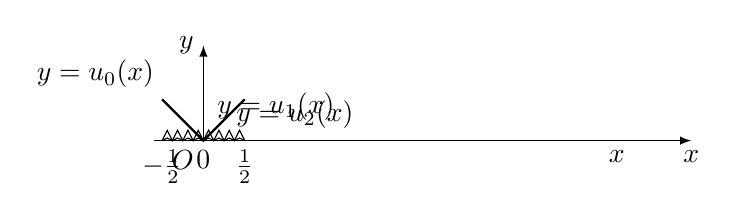
\begin{tikzpicture}[>=latex, scale=1.05]
    \draw[->] (-0.60,0) -- (5.90,0) node[below] {$x$};
    \draw[->] (0,0) -- (0,1.15) node[left] {$y$};
    \node[below left] at (0,0) {$O$};
    % u_0 = |x|（一个 V）
    \draw[thick] (-0.50,0.50) -- (0,0) -- (0.50,0.50);
    \node[above left] at (-0.48,0.52) {$y=u_{0}(x)$};
    \node[below] at (-0.50,0) {$-\frac{1}{2}$};
    \node[below] at (0,0) {$0$};
    \node[below] at (0.50,0) {$\frac{1}{2}$};
    \node[below] at (5.00,0) {$x$};
    % u_1：周期 1/4、高 1/8 的细齿
    \draw[thin] (-0.50,0) -- (-0.4375,0.125) -- (-0.375,0) -- (-0.3125,0.125) -- (-0.25,0)
      -- (-0.1875,0.125) -- (-0.125,0) -- (-0.0625,0.125) -- (0,0)
      -- (0.0625,0.125) -- (0.125,0) -- (0.1875,0.125) -- (0.25,0)
      -- (0.3125,0.125) -- (0.375,0) -- (0.4375,0.125) -- (0.50,0);
    \node[above right] at (0.05,0.13) {$y=u_{1}(x)$};
    % u_2：周期 1/16、高 1/32（只画 4 个齿示意）
    \draw[thin] (-0.50,0) -- (-0.4375,0.03125) -- (-0.375,0) -- (-0.3125,0.03125) -- (-0.25,0)
      -- (-0.1875,0.03125) -- (-0.125,0) -- (-0.0625,0.03125) -- (0,0)
      -- (0.0625,0.03125) -- (0.125,0) -- (0.1875,0.03125) -- (0.25,0)
      -- (0.3125,0.03125) -- (0.375,0) -- (0.4375,0.03125) -- (0.50,0);
    \node[above right] at (0.28,0.033) {$y=u_{2}(x)$};
  \end{tikzpicture}
  \caption{锯齿形函数 $u_{k}(x)=\frac{1}{4^{k}}u_{0}(4^{k}x)$}\label{fig:13.2.5}
\end{figure}

显然, $\forall s\in\mathbb{Z}$, $u_{0}(x)$ 在 $\left[\frac{s}{2},\frac{s+1}{2}\right]$ 上是线性的, 因此, $u_{k}(x)$ 在 $\left[\frac{s}{2\cdot4^{k}},\frac{s+1}{2\cdot4^{k}}\right]$ 上是线性的. 从而每个 $u_{k}(x)$ 都是锯齿形函数, 其齿随 $k$ 增大而变细. 令
\[
  f(x)=\sum_{k=0}^{\infty}u_{k}(x),\quad x\in(-\infty,+\infty).
\]
因为 $|u_{k}(x)|\leqslant\frac{1}{2}\cdot\frac{1}{4^{k}}$, 故由 Weierstrass 判别法, $\sum_{k=1}^{\infty}u_{k}(x)$ 在 $(-\infty,+\infty)$ 上一致收敛. 再由 $u_{k}(x)$ 连续 ($k\in\mathbb{N}$), 根据定理~\ref{thm:13.2.1p} 知, $f(x)=\sum_{k=0}^{\infty}u_{k}(x)$ 在 $(-\infty,+\infty)$ 上处处连续.

下面证明 $f(x)$ 在 $(-\infty,+\infty)$ 上处处不可导.

任取 $x_{0}\in\mathbb{R}$, 记 $[2\cdot4^{n}x_{0}]=s_{n}$, 则
\[
  s_{n}\leqslant2\cdot4^{n}x_{0}<s_{n}+1\Leftrightarrow\frac{s_{n}}{2\cdot4^{n}}\leqslant x_{0}<\frac{s_{n}+1}{2\cdot4^{n}},
\]
取 $x_{n}\in\left[\frac{s_{n}}{2\cdot4^{n}},\frac{s_{n}+1}{2\cdot4^{n}}\right]$, 使得
\[
  \left|x_{n}-x_{0}\right|=\frac{1}{2}\cdot\frac{1}{2\cdot4^{n}}=\frac{1}{4^{n+1}}
\]
(\cref{fig:13.2.6}).

\begin{figure}[htbp]
  \centering
  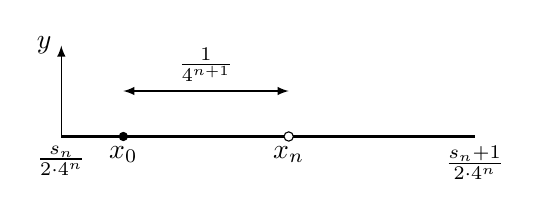
\begin{tikzpicture}[>=latex, scale=1.05]
    \draw[thick] (0,0) -- (5.00,0);
    \draw[->] (0,0) -- (0,1.10) node[left] {$y$};
    \fill (0.75,0) circle (1.6pt);
    \draw[fill=white] (2.75,0) circle (1.6pt);
    \node[below] at (0.75,0) {$x_{0}$};
    \node[below] at (2.75,0) {$x_{n}$};
    \draw[<->] (0.75,0.55) -- (2.75,0.55);
    \node[above] at (1.75,0.55) {$\frac{1}{4^{n+1}}$};
    \node[below] at (0,0) {$\frac{s_{n}}{2\cdot4^{n}}$};
    \node[below] at (5.00,0) {$\frac{s_{n}+1}{2\cdot4^{n}}$};
  \end{tikzpicture}
  \caption{取点 $x_{0}$ 与 $x_{n}$ 的位置}\label{fig:13.2.6}
\end{figure}

\[
  \lim_{n\to+\infty}x_{n}=x_{0}.
\]
于是对某个 $n\in\mathbb{N}$, 当 $k>n$ 时, 有
\[
  \begin{aligned}
    u_{k}(x_{n})&=u_{k}\left(x_{0}\pm\frac{1}{4^{n+1}}\right)=u_{k}\left(x_{0}+\frac{1}{4^{k}}\cdot4^{k-(n+1)}\right)\\
    &\xlongequal{\frac{1}{4^{k}}\text{ 为 }u_{k}\text{ 的周期}}u_{k}(x_{0}),
  \end{aligned}
\]
由此得到
\[
  \begin{aligned}
    \frac{f(x_{n})-f(x_{0})}{x_{n}-x_{0}}&=\sum_{k=0}^{\infty}\frac{u_{k}(x_{n})-u_{k}(x_{0})}{x_{n}-x_{0}}=\sum_{k=0}^{n}\frac{u_{k}(x_{n})-u_{k}(x_{0})}{x_{n}-x_{0}}\\
    &=\sum_{k=0}^{n}(\pm1)=\begin{cases}
      \text{偶数}, & n\text{ 为奇数},\\
      \text{奇数}, & n\text{ 为偶数}
\end{cases}
  \end{aligned}
\]
(当 $k\leqslant n$ 时, $\left[\frac{s_{n}}{2\cdot4^{n}},\frac{s_{n}+1}{2\cdot4^{n}}\right]\subset\left[\frac{s_{k}}{2\cdot4^{k}},\frac{s_{k}+1}{2\cdot4^{k}}\right]$, 而 $u_{k}(x)$ 在 $\left[\frac{s_{k}}{2\cdot4^{k}},\frac{s_{k}+1}{2\cdot4^{k}}\right]$ 中是线性的. 因此, 在 $\left[\frac{s_{n}}{2\cdot4^{n}},\frac{s_{n}+1}{2\cdot4^{n}}\right]$ 上也是线性的. 现 $x_{0},x_{n}\in\left[\frac{s_{n}}{2\cdot4^{n}},\frac{s_{n}+1}{2\cdot4^{n}}\right]$, 所以 $\frac{u_{k}(x_{n})-u_{k}(x_{0})}{x_{n}-x_{0}}=\pm1$.)

令 $n\to+\infty$, 显然有
\[
  \lim_{n\to+\infty}\frac{f(x_{n})-f(x_{0})}{x_{n}-x_{0}}
\]
不存在, 从而 $f(x)$ 在 $x_{0}$ 不可导. 由 $x_{0}$ 的任取性知, $f(x)$ 在 $(-\infty,+\infty)$ 上处处不可导.

\begin{example}[填满正方形的连续曲线]\label{ex:13.2.15}
1890 年, Peano 构造出一条连续曲线, 它将整个正方形填满了. 这一事实就像处处连续处处不可导的函数那样令人不可思议. 下面介绍的例子是 Schoenberg 于 1938 年提出的, 它也需依靠无穷级数来完成.
\end{example}

我们要构造一条连续曲线 $(x,y)=(x(t),y(t))$, $t\in[0,1]$. 当 $t$ 走遍了 $[0,1]$ 时, $(x(t),y(t))$ 连续地走遍正方形 $[0,1]\times[0,1]$ 中每一点. 为此, 在 $[0,1]$ 上定义函数 $\varphi$ 如下:
\[
  \varphi(t)=\begin{cases}
    0, & t\in\left[0,\frac{1}{3}\right],\\
    3t-1, & t\in\left(\frac{1}{3},\frac{2}{3}\right),\\
    1, & t\in\left[\frac{2}{3},1\right].
\end{cases}
\]
然后再将 $\varphi(t)$ 延拓为整个数轴上周期为 $2$ 的偶函数 (\cref{fig:13.2.7}), 即让 $\varphi(t)$ 满足:
\[
  \varphi(t)=\varphi(-t),\quad\varphi(t+2)=\varphi(t),\quad t\in(-\infty,+\infty).
\]

\begin{figure}[htbp]
  \centering
  \begin{tikzpicture}[>=latex, scale=1.10]
    \draw[->] (-0.60,0) -- (8.90,0) node[below] {$x$};
    \draw[->] (0,0) -- (0,2.30) node[left] {$y$};
    \node[below left] at (0,0) {$O$};
    \node[left] at (0,1.90) {$1$};
    \draw[thick] (0,0) -- (1.33,0) -- (2.67,1.90) -- (5.33,1.90) -- (6.67,0) -- (8.00,0);
    \node[below] at (1.33,0) {$\frac{1}{3}$};
    \node[below] at (2.67,0) {$\frac{2}{3}$};
    \node[below] at (5.33,0) {$\frac{4}{3}$};
    \node[below] at (6.67,0) {$\frac{5}{3}$};
    \node[below] at (8.00,0) {$2$};
    \node[above right] at (3.40,1.90) {$y=\varphi(t)$};
  \end{tikzpicture}
  \caption{$\varphi(t)$ 的周期为 $2$ 的偶延拓}\label{fig:13.2.7}
\end{figure}

现在令
\[
  (x(t),y(t))=\biggl(\sum_{n=1}^{\infty}\frac{\varphi(3^{2n-2}t)}{2^{n}},\sum_{n=1}^{\infty}\frac{\varphi(3^{2n-1}t)}{2^{n}}\biggr),\quad t\in[0,1].
\]

这是一条能填满正方形 $[0,1]\times[0,1]$ 的连续曲线.

由于 $0\leqslant\varphi(t)\leqslant1$, 所以 $\sum_{n=1}^{\infty}\frac{1}{2^{n}}$ 是上面两个函数级数的优级数, 根据 Weierstrass 判别法, 得
\[
  x(t)=\sum_{n=1}^{\infty}\frac{\varphi(3^{2n-2}t)}{2^{n}}\quad\text{与}\quad y(t)=\sum_{n=1}^{\infty}\frac{\varphi(3^{2n-1}t)}{2^{n}}
\]
在 $[0,1]$ 上都一致收敛, 根据定理~\ref{thm:13.2.1p}, $x(t)$ 与 $y(t)$ 都为 $[0,1]$ 上的连续函数, 所以, $(x(t),y(t))$ 是一条连续曲线. 余下的需证它填满了整个正方形 $[0,1]\times[0,1]$. 为此, 任取 $(a,b)\in[0,1]\times[0,1]$, 并且用二进位小数表示 $a,b$ 为
\[
  a=\sum_{n=1}^{\infty}\frac{a_{n}}{2^{n}},\quad b=\sum_{n=1}^{\infty}\frac{b_{n}}{2^{n}},
\]
这里 $a_{n},b_{n}$ 都只取 $0,1$ 中某一个值, 将 $\{a_{n}\}$, $\{b_{n}\}$ 交错排列为
\[
  a_{1},b_{1},a_{2},b_{2},\cdots,a_{n},b_{n},\cdots,
\]
并重新记为
\[
  \eta_{1},\eta_{2},\cdots,\eta_{2n-1},\eta_{2n},\cdots,
\]
其中 $\eta_{2n-1}=a_{n}$, $\eta_{2n}=b_{n}$, $n=1,2,\cdots$, 于是
\[
  0\leqslant\eta=\sum_{n=1}^{\infty}\frac{2\eta_{n}}{3^{n}}\leqslant2\sum_{n=1}^{\infty}\frac{1}{3^{n}}=1,
\]
即 $\eta\in[0,1]$. 我们证 $(x(\eta),y(\eta))=(a,b)$. 事实上, 对于固定的 $k=0,1,2,\cdots$, 有
\[
  3^{k}\eta=3^{k}\sum_{n=1}^{\infty}\frac{2\eta_{n}}{3^{n}}=2\sum_{n=1}^{k}3^{k-n}\eta_{n}+\frac{2}{3}\eta_{k+1}+2\sum_{n=k+2}^{\infty}\frac{\eta_{n}}{3^{n-k}}.
\]
容易看出, 右边第 1 个和式是 $2$ 的整倍数, 记为 $2m$. 若将第 3 个和式记为 $\alpha_{k}$, 则
\[
  0\leqslant\alpha_{k}\leqslant2\sum_{n=k+2}^{\infty}\frac{1}{3^{n-k}}=\frac{1}{3}.
\]
这样便有
\[
  3^{k}\eta=2m+\frac{2}{3}\eta_{k+1}+\alpha_{k}.
\]
由于 $\varphi(t)$ 是以 $2$ 为周期的周期函数, 所以
\[
  \begin{aligned}
    \varphi(3^{k}\eta)&=\varphi\left(2m+\frac{2}{3}\eta_{k+1}+\alpha_{k}\right)\\
    &=\varphi\left(\frac{2}{3}\eta_{k+1}+\alpha_{k}\right)=\begin{cases}
      \varphi(\alpha_{k})=0=\eta_{k+1}, & \eta_{k+1}=0,\\
      \varphi\left(\frac{2}{3}+\alpha_{k}\right)=1=\eta_{k+1}, & \eta_{k+1}=1
\end{cases}\\
    &=\eta_{k+1},
  \end{aligned}
\]
其中 $\eta_{k+1}=1$ 时, $\frac{2}{3}\leqslant\frac{2}{3}\eta_{k+1}+\alpha_{k}\leqslant\frac{2}{3}\cdot1+\frac{1}{3}=1$. 于是
\[
  x(\eta)=\sum_{n=1}^{\infty}\frac{\varphi(3^{2n-2}\eta)}{2^{n}}=\sum_{n=1}^{\infty}\frac{\eta_{2n-1}}{2^{n}}=\sum_{n=1}^{\infty}\frac{a_{n}}{2^{n}}=a,
\]
\[
  y(\eta)=\sum_{n=1}^{\infty}\frac{\varphi(3^{2n-1}\eta)}{2^{n}}=\sum_{n=1}^{\infty}\frac{\eta_{2n}}{2^{n}}=\sum_{n=1}^{\infty}\frac{b_{n}}{2^{n}}=b.
\]
这就证明了连续曲线 $(x(t),y(t))$ 的确填满了整个正方形 $[0,1]\times[0,1]$.

\begin{remark}\label{rem:13.2.2}
注意映射 $F\colon[0,1]\to[0,1]\times[0,1]$, $t\to F(t)=(x(t),y(t))$ 肯定不是一一映射, 当然更不是同胚映射. 这表明: 必有 $t_{1},t_{2}\in[0,1]$, $t_{1}\neq t_{2}$, 但 $F(t_{1})=(x(t_{1}),y(t_{1}))=(x(t_{2}),y(t_{2}))=F(t_{2})$, 称它为重点.

事实上, 若映射 $F$ 为一一映射, 根据\extref{定理 7.3.10} 知, 该映射必为同胚映射. 从而也为同胚. 而 $[0,1]\setminus\left\{\frac{1}{2}\right\}=\left[0,\frac{1}{2}\right)\cup\left(\frac{1}{2},1\right]$ 不连通, 而 $[0,1]\times[0,1]\setminus F\left(\frac{1}{2}\right)$ 连通, 这与连通为同胚不变性相矛盾.

不难看出, 利用上面的方法, 我们还能构造出填满整个立方体 $[0,1]\times[0,1]\times[0,1]$ 的空间连续曲线. 请读者证明, 空间连续函数
\[
  F(t)=(x(t),y(t),z(t))=\left(\sum_{n=1}^{\infty}\frac{\varphi(3^{3n-3}t)}{2^{n}},\sum_{n=1}^{\infty}\frac{\varphi(3^{3n-2}t)}{2^{n}},\sum_{n=1}^{\infty}\frac{\varphi(3^{3n-1}t)}{2^{n}}\right)
\]
便能填满整个立方体 $[0,1]\times[0,1]\times[0,1]$. 同样 $F\colon[0,1]\to[0,1]\times[0,1]\times[0,1]$ 也不是一一映射, 即上述空间连续曲线必有重点.
\end{remark}

上述例~\ref{ex:13.2.14} 与例~\ref{ex:13.2.15} 两个例子的魅力不仅在于它们提示了两件令人感到惊异的事实. 还在于它们是近 20 年来正蓬勃兴起并且很有应用前景的一门新兴学科 ``分形几何'' 中所谓 ``分形集'' 的典型例子.

\begin{exblock}{练习题 13.2}
\begin{enumerate}
  \item 确定下列函数的存在域, 并研究它们的连续性:
  \begin{enumerate}
    \item $f(x)=\displaystyle\sum_{n=1}^{\infty}\left(x+\frac{1}{n}\right)^{n}$;
    \item $f(x)=\displaystyle\sum_{n=1}^{\infty}\frac{x+(-1)^{n}n}{x^{2}+n^{2}}$.
  \end{enumerate}
  \item 证明: 函数
  \[
    f(x)=\sum_{n=1}^{\infty}\frac{\cos nx}{n^{4}}
\]
  在 $(-\infty,+\infty)$ 中有二阶连续导函数, 并计算 $f''(x)$.
  \item 设 $f(x)=\sum_{n=1}^{\infty}n\mathrm{e}^{-nx}$ ($x>0$), 计算 $\int_{\ln2}^{\ln3}f(x)\mathrm{d}x$.
  \item 设 $f(x)=\sum_{n=1}^{\infty}\left(\frac{x}{1+2x}\right)^{n}\cos\frac{n\pi}{x}$, 计算: $\lim\limits_{x\to1}f(x)$, $\lim\limits_{x\to+\infty}f(x)$.
  \item 已知 $\sum_{n=1}^{\infty}\frac{(-1)^{n-1}}{n}=\ln2$, 证明: $\lim\limits_{x\to1}\sum_{n=1}^{\infty}\frac{(-1)^{n-1}}{n^{x}}=\ln2$.
  \item 证明: $f(x)=\sum_{n=1}^{\infty}\left(x+\frac{1}{n}\right)^{n}$ 在 $(-1,1)$ 内连续.
  \item 证明: $\sum_{n=1}^{\infty}\frac{x}{(1+x^{2})^{n}}$ 在 $(0,+\infty)$ 内非一致收敛.
\end{enumerate}
\end{exblock}

\begin{exblock}{思考题 13.2}
\begin{enumerate}
  \item 设 $E$ 为 $(-\infty,+\infty)$ 中的一点集, $x_{0}$ 为 $E$ 的广义聚点 (即 $x_{0}$ 可为实数或 $\pm\infty$, $x_{0}$ 的任何开邻域中必含 $E$ 中异于 $x_{0}$ 的点). 如果函数项级数 $\sum_{n=1}^{\infty}u_{n}(x)$ 在 $E$ 上一致收敛, 且 $\lim\limits_{n\to+\infty}u_{n}(x)=a_{n}$, $n=1,2,\cdots$. 证明:

  (1) $\sum_{n=1}^{\infty}a_{n}$ 收敛;

  (2) $\lim\limits_{x\to x_{0}}\sum_{n=1}^{\infty}u_{n}(x)=\sum_{n=1}^{\infty}a_{n}=\sum_{n=1}^{\infty}\lim\limits_{x\to x_{0}}u_{n}(x)$.
  \item 利用 $\sum_{n=1}^{\infty}\frac{1}{n^{2}}=\frac{\pi^{2}}{6}$, 证明:
  \[
    \lim_{x\to1}\sum_{n=1}^{\infty}\frac{x^{n}(1-x)}{n(1-x^{2n})}=\frac{\pi^{2}}{12}.
\]
  \item 设函数项级数 $\sum_{n=1}^{\infty}u_{n}(x)$ 满足下列条件:

  (1) $\sum_{n=1}^{\infty}u_{n}(x)$ 在 $(x_{0}-\delta,x_{0}+\delta)$ 中收敛于 $f(x)$;

  (2) 函数项级数的每一项 $u_{n}(x)$ 在 $x=x_{0}$ 处可导;

  (3) 函数项级数 $\sum_{n=1}^{\infty}\frac{u_{n}(x)-u_{n}(x_{0})}{x-x_{0}}$ 在 $0<|x-x_{0}|<\delta$ 中一致收敛.

  则 $f(x)$ 在 $x_{0}$ 处可导, 且 $f'(x_{0})=\sum_{n=1}^{\infty}u_{n}'(x_{0})$.
  \item 在 $(0,1)$ 中任取一数列 $\{a_{n}\}$, 其中两两不相同. 证明: 函数
  \[
    f(x)=\sum_{n=1}^{\infty}\frac{|x-a_{n}|}{2^{n}}
\]
  在 $(0,1)$ 中连续, 且在 $x=a_{n}$ ($n=1,2,\cdots$) 处都不可导, 而在 $(0,1)$ 中其他点处都可导.
  \item 设 $\{x_{n}\}$ 为区间 $[0,1)$ 中的全体有理数, 对任意 $x\in(0,1)$, 定义
  \[
    f(x)=\sum_{x_{n}<x}\frac{1}{2^{n}}.
\]
  令
  \[
    g_{n}(x)=\begin{cases}
      0, & x\leqslant x_{n},\\
      \frac{1}{2^{n}}, & x>x_{n},
\end{cases}
\]
  证明:

  (1) 级数 $\sum_{n=1}^{\infty}g_{n}(x)$ 在 $(0,1)$ 上一致收敛于 $f(x)$;

  (2) $\int_{0}^{1}f(x)\mathrm{d}x=\sum_{n=1}^{\infty}\frac{1-x_{n}}{2^{n}}$.
  \item 设 $\{x_{n}\}$ 为 $(0,1)$ 内的一个数列, 且 $x_{i}\neq x_{j}$ ($i\neq j$), 证明
  \[
    f(x)=\sum_{n=1}^{\infty}\frac{\operatorname{sgn}(x-x_{n})}{2^{n}}
\]
  在 $(0,1)$ 内一致收敛; $f(x)$ 在 $(0,1)\setminus\{x_{n}\mid n=1,2,\cdots\}$ 中每一点处连续, 而在每个 $x_{n}$ ($n=1,2,\cdots$) 处不连续.
  \item 证明: $f(x)=\sum_{n=1}^{\infty}n\mathrm{e}^{-nx}$ 在 $(0,+\infty)$ 内收敛, 但不一致收敛, 而和函数在 $(0,+\infty)$ 内无穷次可导.
  \item 设 $h(x)$, $f_{n}'(x)$ 在 $[a,b]$ 上连续, $n=1,2,\cdots$, 又对 $[a,b]$ 中任意的 $x_{1},x_{2}$ 与正整数 $n$ 有
  \[
    \left|f_{n}(x_{1})-f_{n}(x_{2})\right|\leqslant\frac{M}{n}|x_{1}-x_{2}|,
\]
  其中 $M\geqslant0$ 为常数. 证明:

  (1) $f_{n}'(x)\rightrightarrows0$, $x\in[a,b]$, $n\to+\infty$;

  (2) $\lim\limits_{n\to+\infty}\int_{a}^{b}h(x)f_{n}'(x)\mathrm{d}x=0$.
\end{enumerate}
\end{exblock}
